\section{Introduction}
\label{sec:intro}

With the publications of the first ever observation of $\nu_e$ appearance, and the world's most precise measurement of $\theta_{23}$, T2K has achieved its initial experimental goals with only 8.5\% of the approved protons on target (POT). The next phase of the experiment will make even more precise measurements of $\nu_e$ appearance and $\nu_\mu$ disappearance using both neutrinos and anti-neutrinos in order to probe the value of $\delta_{CP}$, the $\theta_{23}$ octant, and $\left|\Delta m^2_{32}\right|$. In conjunction with measurements from NO$\nu$A, these measurements may also provide a constraint on the neutrino mass hierarchy.

In order to achieve these goals, a more precise understanding of neutrino interaction cross sections is required. Currently, T2K is forced to rely on neutrino interaction generators to translate experimental observables into constraints on the neutrino energy spectrum, which depends on the value of the oscillation parameters. Measurements of very forward-going muons on the carbon target employed by the existing near detector, ND280, are translated into constraints on the 4$\pi$ muon angular distribution on a water target seen at the far detector. The interactions of final-state hadrons both within the nucleus and within each detector medium can have a significantly different impacts on the near and far detector analyses. Some of the backgrounds at far detector, Super-Kamiokande (Super-K), are poorly constrained at ND280. This is particularly true of NC$\pi^+$ events, which are problematic both because the cross section is not well measured, and because $\pi^+$ reconstruction at Super-K is not well understood. This results in a contamination of both the $\nu_\mu$ and $\nu_e$ samples that produces large systematic uncertainties.

It is also necessary to measure events with single, electron-like rings in order to constrain any differences in the \nue and \numu cross sections. These events can be caused by a variety of sources, such as beam $\nu_e$, single $\gamma$ production, $\pi^0$ production, external $\gamma$ background, sterile neutrino oscillations and radiative muon production. An excess of such events has been observed by MiniBooNE. It is important to confirm whether a similar excess exists on a water target, ideally with a water Cherenkov detector, and if found, the cause must be understood in order to perform precision \nue appearance measurements.

The least constrained component of these neutrino interaction models, however, is the relationship between the experimentally observable lepton kinematics and the energy of the incident neutrino. At present, there is an experimentally-unconstrained and potentially large bias in the ability to translate lepton kinematics to neutrino energy. Current estimates, based solely on new, recently developed models, suggest that this bias may be one of T2K's largest systematic uncertainties, and no existing dataset can provide a constraint on this uncertainty in a manner that does not rely on neutrino interaction models. Had neutrino interaction models been trusted to provide this relationship just 5 years ago, current models suggest that 20 to 30\% of events where only the final state lepton was observed would have been reconstructed with an incorrect neutrino energy in a way that would not have been constrained or even detectable. Even a high-performance near detector, capable of precisely measuring all charged particles in the final state, would be forced to rely on models that relate lepton kinematics to hadronic final states, and no modern theoretical models offer a prediction for such a relationship within a nuclear environment.

%The obvious solution to constrain the final state particle kinematics for interactions at a fixed neutrino energy is the use of a monochromatic neutrino beam.  In principle, such beams could be made using the two-body decays from a monochromatic charged pion beam, but such a beam is inefficient and technically challenging to build.  In a conventional neutrino beam, the peak neutrino energy varies with the angle between the neutrino direction and average pion direction, off-axis angle, and the neutrino spectrum becomes narrower at larger off-axis angles.  This energy dependence with off-axis angle can be used to over-constrain the relationship between observed final state particle kinematics and predicted neutrino spectra in a manner not possible with measurements at a single off-axis angle.

The nuPRISM water-Cherenkov detector takes advantage of the energy dependence of the neutrino flux with off-axis angle by spanning a continuous range of 1 to 4 degrees in off-axis angle.
%The \nuprism neutrino detection principle provides a mechanism whereby the far detector response for any given oscillation hypothesis can be directly measured at the near detector. 
%The \nuprism concept involves a 50-60 m tall water-Cherenkov detector located about 1 km from the T2K neutrino production point, covering an off-axis angle range of 1-4$^{\circ}$.
This technique has the potential to significantly reduce uncertainties from neutrino interaction modeling in T2K oscillation analyses, as is demonstrated for the muon neutrino disappearance measurement described in Section~\ref{sec:physics}. In particular, these measurements will provide the first direct experimental constraint on the relationship between lepton kinematics and neutrino energy using measurements of final state muons at many different off-axis angles.
 In order to construct a more cost-effective detector that can reasonably be built on a timescale that is applicable to T2K, this document proposes to instrument a subset of the full water volume on a frame that moves vertically within the water tank, which sequentially samples the full off-axis range of the shaft in 5-6 separate running periods.

The construction of a \nuprism detector in the next 3-5 years can also provide significant benefits to Hyper-Kamiokande (Hyper-K). The problems with understanding neutrino interactions can have a larger impact on Hyper-K, since Hyper-K will have much smaller statistical errors, and a demonstration that these uncertainties can be managed with a \nuprism near detector will significantly enhance the physics case for Hyper-K.
In addition, \nuprism is an easily accessible water Cherenkov detector that provides an ideal environment to test Hyper-K technology. Hyper-K proposes to use new, in-water electronics, new solid state hybrid-PMTs (HPDs), and a new tank and liner construction to prevent leaks, all of which require extensive testing in a prototype detector.
Finally, \nuprism will provide an intermediate physics program that bridges the gap from T2K phase I to Hyper-K, which can provide continuity within the Japanese physics community while Hyper-K is being designed and constructed.

The remainder of this document provides an overview of the detector components and physics potential of \nuprism. The results for a full T2K $\nu_\mu$ disappearance analysis are provided, and a variety of additional \nuprism neutrino energy spectrum fits are presented to demonstrate how the \nuprism technique can constrain \nue cross sections, which will be important for measurements of $\nu_e$ appearance and $\delta_{CP}$, as well as several different oscillation backgrounds. Cost estimates have been obtained for the items that are expected to dominate the cost of the project, in particular photomultiplier tubes (PMTs) and civil construction. For the additional less expensive items, cost estimates from a very similar project proposed in 2005, the T2K 2~km water Cherenkov detector, are used to guide expectations for the full \nuprism project cost.

\subsection{\label{sec:enu_determine}Uncertainties in Neutrino Energy Determination}

Prior to 2009, neutrino interaction models assumed that neutrinos, when encountering a nuclear target, interact a single nucleon. The initial state of the nucleon was characterized by a binding energy and Fermi momentum, which were drawn from either a Fermi gas~\cite{LlewellynSmith:1971zm,Smith:1972xh} or a more specialized spectral function treatment~\cite{Benhar:1989aw}. In this paradigm, all the remaining dynamics of charge-current quasi-elastic (CCQE) interactions, in which the target neutron is converted into an outgoing proton, are encapsulated in a set of three vector and three axial-vector form factors. Most of these form factors are tightly constrained from external electron and pion scattering experiments (for a detailed discussion, see Ref.~\cite{nue-numu-cross-section}). The largest remaining uncertainty is on the axial vector form factor, which is assumed to take a dipole form,
\begin{equation}
F_A(Q^2)=\frac{F_A(0)}{(1+\frac{Q^2}{M_A^2})^2}.
\end{equation}
The parameter $F_A(0)$ is precisely known from nuclear beta decay, which leaves $M_A$ as the remaining uncertain parameter. Modifying $M_A$ simultaneously alters both the overall CCQE cross section and the shape of the $Q^2$ distribution.

In 2009, the first comparison of MiniBooNE CCQE-like data at neutrino energies around 1~GeV and NOMAD data at higher energies was released. A reproduction of that comparison 
%with LSND and SciBooNE data included 
is shown in Figure~\ref{fig:miniboonenomad}. The MiniBooNE data are consistent with an $M_A$ value of 1.35~GeV (an additional empirical parameter, $\kappa$ is consistent with no modification at $1~\sigma$), while the NOMAD data prefer an $M_A$ of 1.03~GeV. 
This discrepancy is currently unexplained by neutrino-nucleus interaction models and is an outstanding experimental question that can be addressed by nuPRISM (see Section~\ref{sec:cc0pi}).
%This discrepancy could not be explained using the neutrino-nucleus interaction models available at that time.

\begin{figure*}[htpb]
     \begin{center}
       %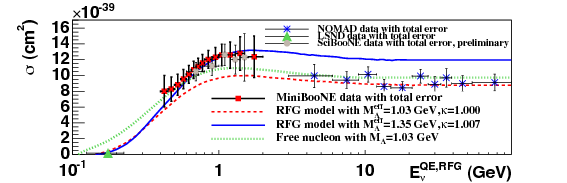
\includegraphics[width=15cm]{figures/enu_xsec_mb_sb_lsnd_nomad.png}
       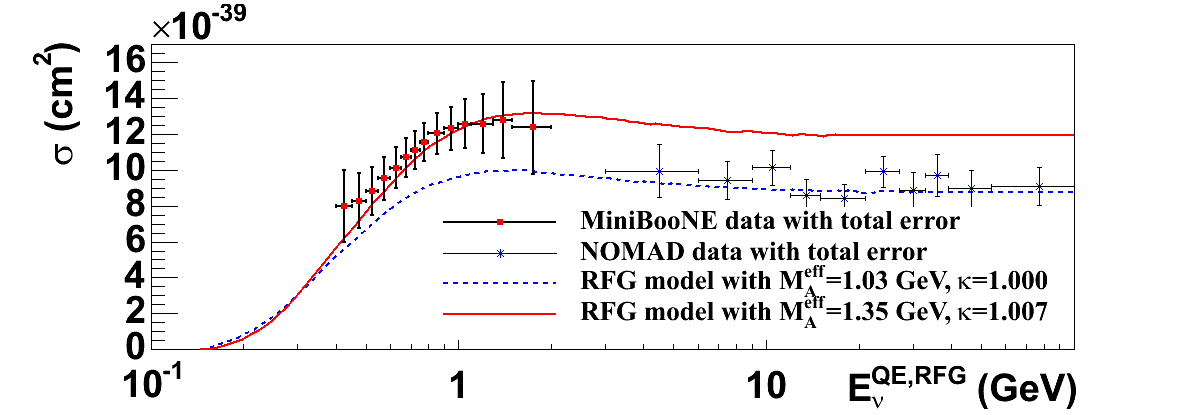
\includegraphics[width=15cm]{figures/sigma_sam.png}
       \caption{The CCQE cross section measurements are shown for MiniBooNE and NOMAD. The data show significant differences between measurements made at low and high energies.}
     \end{center}
\label{fig:miniboonenomad}
\end{figure*}

Later in 2009, the Marteau~\cite{Marteau:1999kt} formalism for the treatment of neutrino scattering on nucleon 
pairs in nuclei was resurrected by Martini {\it et al.}~\cite{Martini:2009uj,Martini:2010ex,Martini:2011wp} to explain the
 higher event rate and muon kinematic distributions observed by MiniBooNE.  If this explanation of the MiniBooNE event 
excess were correct, it would imply that neutrino energy reconstruction for all previous neutrino experiments on nuclei
 at the GeV scale could have significant biases for 20-30\% of CCQE-like events. In the past few years, the models of Martini {\it et al.} and Nieves {\it et al.}~\cite{Nieves:2011pp} have begun to incorporate these effects, but such calculations are very difficult and the predictions of just these two models produce significantly different results when applied to T2K oscillation analyses~\cite{TN172}.
 
There exists circumstantial experimental evidence for multinucleon interaction mechanisms in both neutrino and electron scattering, but nothing that allows us to conclusively solve the problem or even to down-select among the various calculations.  In electron scattering, the reaction mechanism is different due to the absence of an axial-vector current component.  In neutrino scattering experiments with broadband beams, the evidence is only circumstantial, since we must rely on the predictions of the models themselves to extract the neutrino energy for any given event. Other approaches, such as making precise measurements of the hadronic final state, are limited by a lack of theoretical understanding of the expected hadron kinematics for multinucleon events. Even the final state hadron spectra for CCQE events are modified by nuclear effects which are also not well understood.

Figure~\ref{fig:badnd} illustrates the challenge associated with using near detector data to constrain the interaction model that predicts far detector event rates. The detectors measure the convolution of the neutrino spectrum with the interaction model.  Since the near and far detector spectra are different due to neutrino oscillations, the measurement of this convolution in the near detector does not directly constrain the event rate in the far detector, and neutrino energies that represent a small fraction of the event rate in the near detector can be a significantly impact the measurement of oscillation parameters in the far detector.
%Figure~\ref{fig:badnd} illustrates the difficulties associated with using near detectors to constrain the effects of neutrino interaction modeling on the predictions for a far detector.

In addition to multinucleon effects, other effects such as long range correlations and final state interactions within the target nucleus can also produce distortions to the neutrino energy spectrum that can be difficult to model. In order to perform precision oscillation measurements with uncertainties at the level of the few percent statistical errors expected for $7.8\times10^{21}$ POT, it will be necessary to provide a data-driven constraint on these neutrino interaction model uncertainties.

\begin{figure}[htpb]
     \begin{center}
       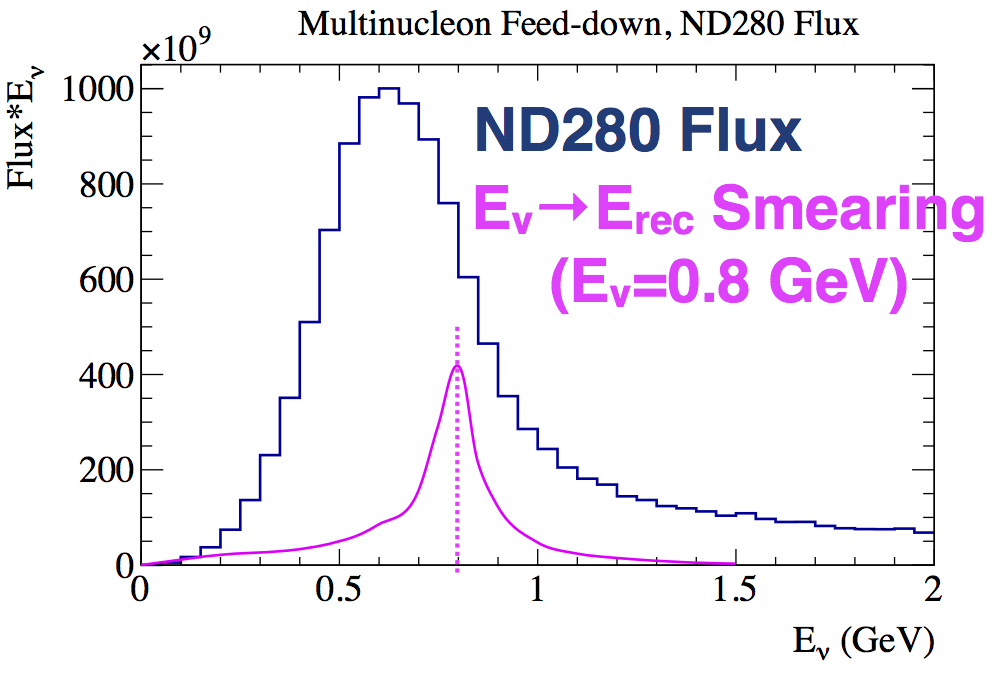
\includegraphics[width=7cm]{figures/MartiniFeedDownND280_2.png}
       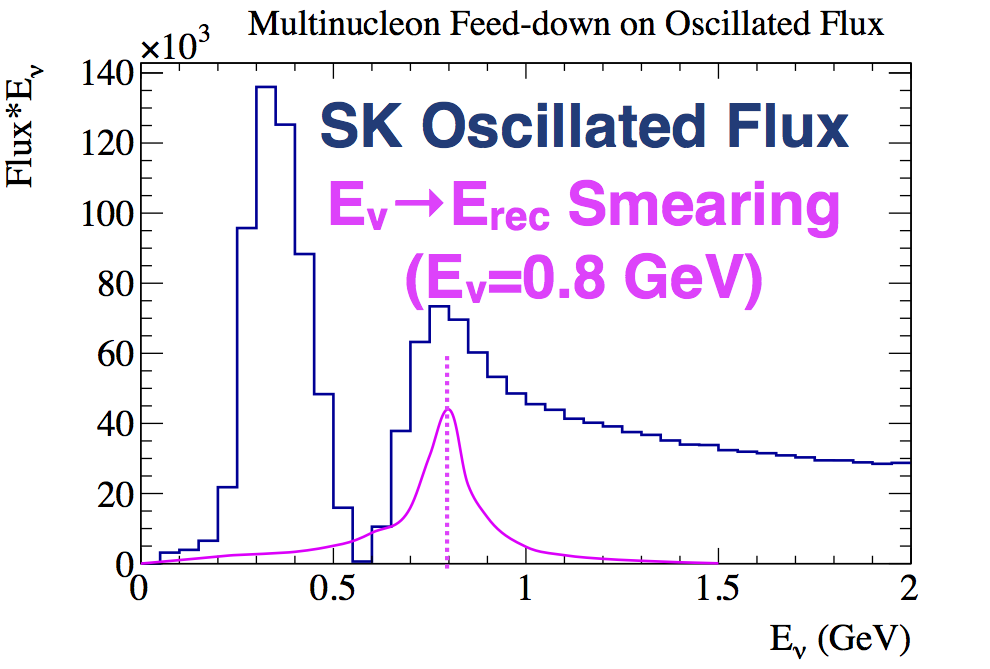
\includegraphics[width=7cm]{figures/MartiniFeedDownSK_2.png}
       \caption{A cartoon of the effect of energy reconstruction biases is shown for both the T2K near detector (top) and the far detector (bottom). At the far detector, these biases directly impact the measurement of the oscillation dip, but the biases are largely unconstrained at the near detector due to the large unoscillated sample of unbiased CCQE events.}
       \label{fig:badnd}
     \end{center}
\end{figure}

\subsection{ND280 Capabilities and Limitations}

T2K oscillation analyses rely on precise constraints of flux and cross section model parameters from ND280. While a 3.2\% uncertainty on the predicted number of electron neutrinos at the far detector has been achieved for the combination of flux and cross section parameters that are currently constrained by the near detector, there remains a 4.7\% uncertainty on the far detector event sample due to additional cross section parameters that remain unconstrained. This unconstrained uncertainty is dominated by uncertainties in the modeling of the target oxygen nucleus, and largely depends on the theoretical model used to extrapolate measurements on carbon to oxygen.

The full capabilities of the T2K near detector have not yet been exploited. For example, the near detector analyses have thus far used interactions in the most-upstream Fine-Grained Detector (FGD1), which is composed entirely of alternating layers of horizontally- and vertically-oriented scintillator bars. Since the FGD scintillator layers are predominantly composed of carbon and hydrogen, FGD1 measurements cannot directly probe interactions on oxygen. An additional FGD (FGD2) contains layers of water interspersed within its scintillator layers. A simultaneous fit of the interactions in both FGDs can provide a constraint on nuclear uncertainties in oxygen, and may potentially reduce the corresponding nuclear model uncertainties.
%The ultimate event samples in both FGDs are shown in Table~\ref{tab:futurerates}.
%The statistical precision of a subtraction of interactions on scintillator from interactions on water is better than 1\%, which is more precise current detector systematic uncertainties ($\sim$3\%).

Another expected improvement to ND280 is the extension of the measured phase space of the outgoing lepton kinematics from a charged-current neutrino interaction. In the currently available analyses, muons are required to be produced in an FGD and traverse a minimum distance through the downstream TPC in order to make a measurement of both muon momentum and particle identification. This limits the muon acceptance to forward angles. Improvements to detector timing calibration and to track matching to the Electromagnetic Calorimeters (ECALs) and Side Muon Range Detectors (SMRDs) surrounding the FGDs and TPCs will allow for the reconstruction of charged-current events with backward-going and sideways-going muons. These additional samples will add less than 20\% to the total even sample with a degraded energy resolution relative to events that enter a TPC, however they may be able to improve constraints on the cross section modeling in previously inaccessible and potentially important new regions of phase space.

An additional sample of events that has not yet been incorporated into the oscillation analysis are charged-current interactions in the pi-zero detector (P0D). The P0D is capable of operating with and without water targets dispersed throughout its active volume, and by measuring the event rates separately in these two configurations, it is possible to extract constraints on interactions in water. The requirement to match a track in the TPC limits the angular acceptance for muons produced in the P0D, however the larger fiducial volume of the P0D produces a higher event sample.

In order for any of these new samples to reduce systematic uncertainties, it is necessary to choose a neutrino interaction model that can characterize all possible variations of the neutrino cross sections as a function of both neutrino energy and the final state particle kinematics. In other words, model dependent choices will have to be made that will directly impact the strength of the constraint that can be extracted. Given the difficulties in understanding neutrino-nucleus interactions, it may not be possible to justify reductions in cross section systematic uncertainties beyond their current level without a direct experimental constraint. In addition, the aforementioned uncertainties due to multinucleon effects have not yet been incorporated into T2K oscillation analyses. Preliminary studies within T2K indicate that these effects would be difficult to constrain using only lepton kinematics from ND280 at the level required for the full-statistics T2K sensitivity, and may be as large as the current dominant systematic uncertainties. The use of additional hadronic information is being explored, but any such constraint would be subject to even further model dependence.

\subsection{Detector Overview}

The \nuprismlite detector uses the same water Cherenkov detection technology as Super-K with a cylindrical water volume that is taller than Super-K (50-100~m vs 41~m) but with a much smaller diameter (10-12~m vs 39~m). The key requirements are that the detector span the necessary off-axis range (1$^\circ$-4$^\circ$) and that the diameter is large enough to contain the maximum required muon momentum. The baseline design considers a detector location that is 1~km downstream of the neutrino interaction target with a maximum contained muon momentum of 1~GeV/c. This corresponds to a 50~m tall tank with a 6~m diameter inner detector (ID) and a 10~m diameter outer detector (OD). A larger, 8~m ID is also being considered at the expense of some OD volume at the downstream end of the tank. As the \nuprismlite analysis studies mature, the exact detector dimensions will be refined to ensure sufficient muon momentum, \nue statistics and purity, etc.

The instrumented portion of the tank is a subset of the full height of the water volume, currently assumed to be 10~m for the ID and 14~m for the OD. The novel feature of this detector is the ability to raise and lower the instrumented section of the tank in order to span the full off-axis range in 6 steps. The inner detector will be instrumented with either 5-inch or 8-inch PMTs to ensure sufficient measurement granularity for the shorter light propagation distances relative to Super-K. Also under consideration is to replace the OD reflectors with large scintillator panels, such as those used in the T2K Side Muon Range Detector (SMRD), although this has not yet been integrated into the overall detector design. More details regarding the detector hardware can be found in Section~\ref{sec:detector}



%The expected P0D event rates are given in Table~\ref{tab:futurerates}.

%\begin{table}
%\begin{tabular}{|c|c|c|c|} \hline
%\multicolumn{2}{|c|}{\multirow{3}{*}{Event Sample}} & Total & Right-Sign Event \\
%\multicolumn{2}{|c|}{} & Event Rate & Rate on Water \\
%\multicolumn{2}{|c|}{} & (T2K, TH2K) & (T2K, T2HK) \\ \hline \hline
%\multirow{4}{*}{$\nu$-mode} & FGD1 & (169,000,) & (0,0) \\
%& FGD2 & (166,000,) & (84,000,)   \\
%& P0D Water Out & (144,000,) & (0,0)   \\
%& P0D Water In & (210,000,) & (66,000,) \\ \hline
%\multirow{4}{*}{$\bar{\nu}$-mode} & FGD1 & (57,000,) & (0,0)   \\
%& FGD2 & (56,000,) & (28,000,)   \\
%& P0D Water Out & (63,000,) & (,)   \\
%& P0D Water In & (93,000,) & (30,000,)   \\ \hline
%\end{tabular}
%\caption{The number of selected CC-Inclusive events in FGD1, FGD2, and the P0D are given for the ultimate expected POT assuming 50\% $\nu$-mode horn operation and 50\% $\bar{\nu}$-mode for T2K, and 30\% $\nu$-mode and 70\% $\bar{\nu}$-mode for T2HK. The subset of events that are right-sign interactions (i.e. $\nu$-interactions in $\nu$-mode and $\bar{\nu}$ interactions in $\bar{\nu}$-mode) on water are shown separately.\label{tab:futurerates}}
%\end{table}



%\subsection{Desired Capabilities for an Upgraded Near Detector}
%
%In order to address the challenges T2K will face in making precision oscillation measurements, several enhancements to the currently available near detector capabilities are desirable. The main requirement is to impose a constraint on the relationship between lepton kinematics and neutrino energy, which is currently an unknown and potentially large systematic uncertainty. Since the largest systematic uncertainties in current T2K analyses come from extrapolations of measurements on Carbon to Oxygen, it is also important for the detector to provide a water target. In order to constraint the full phase space of interactions measured at Super-K, it is necessary for the detector to have $4\pi$ detector acceptance, and to have the capability to constrain the various sources of single-ring electron-like events, which requires good e/$\mu$ and e/$\pi^0$ separation. The ability to precisely measure neutral current backgrounds, such as NC$\pi^+$ and NC$\pi^0$, would also provide a significant reduction in systematic uncertainties in T2K oscillation analyses. Finally, it would be preferable to have some sign selection in an upgraded near detector to distinguish neutrino-induced background when the beam is taken with the horn in anti-neutrino mode. In principle, the current ND280 has this capability, so this may not be a strict requirement for a new T2K near detector.

%\begin{itemize}
%\item Provide constraints on neutrino energy construction
%\item water target
%\item 4pi acceptance
%\item Good e/mu, e/pi0 separation
%\begin{itemize}
%\item Provide a measurement of \nue cross sections
%\end{itemize}
%\item Background measurements (NCpi0, NCpi+, ...), preferably as a function of neutrino energy.
%\item Sign selection (perhaps can extrapolate from ND280)
%\end{itemize}

%\clearpage
